\section{Complete analytical details}
\label{app:proofs}

This supplement gives the complete internal derivations behind
Sec.~\ref{sec:response} and Sec.~\ref{sec:estimator}.  They are recorded for
correctness and reproducibility.  As established by the closest-primary-result
audit in Table~\ref{tab:novelty}, the full-probability result is a direct
specialization of circuit-Fourier theory and the observable result is a short
synthesis of the known IQP active-generator expansion with the real-input
filter.  The proofs below are not presented as priority claims.

\subsection{Proof of Proposition~\ref{prop:full-support}}

The density operator of one encoded qubit is
\begin{equation}
 \rho_i(\alpha_i)=R_Y(\alpha_i)|0\rangle\!\langle0|R_Y(\alpha_i)^\dagger
 =\frac12\left(I+\sin\alpha_iX+\cos\alpha_iZ\right).
 \label{eq:local-rho}
\end{equation}
Every matrix entry of Eq.~\eqref{eq:local-rho} is a linear combination of the
three angle frequencies $-1,0,+1$.  Tensoring the local states therefore gives
fixed matrices $A_s$ such that
\begin{equation}
 \rho(c)=\bigotimes_i\rho_i(\alpha_i(c))
 =\sum_{s\in\{-1,0,1\}^n}A_s
 e^{i\sum_i s_i\alpha_i(c)}.
\end{equation}
Substituting $\alpha_i(c)=b_i+w_i^\mathsf{T}c$ absorbs the bias into the
coefficient:
\begin{equation}
 \rho(c)=\sum_s\left(A_se^{i\sum_i s_ib_i}\right)
 e^{i(\sum_i s_iw_i)^\mathsf{T}c}.
\end{equation}
For a fixed unitary $U$ and outcome $x$,
\begin{equation}
 q(x\mid c)=\operatorname{Tr}\!\left[
 U^\dagger|x\rangle\!\langle x|U\rho(c)\right]
\end{equation}
is a fixed linear functional of $\rho(c)$, so it introduces no new frequency.
There are at most three choices per nonzero row of $W$.  Zero rows, coincident
signed sums, and coefficient cancellations only shrink the realized set,
which proves Eqs.~\eqref{eq:full-support}--\eqref{eq:omega-full}.

The proof does not use the IQP structure.  It also does not give an efficient
method for evaluating the trace coefficient $Q_{x,s}$; exact evaluation can
still scale as $2^n$.

\subsection{Proof of Proposition~\ref{prop:observable}}

The final Hadamards map the measured operator to $X_a$.  A diagonal generator
with $a\cdot g_j=0\pmod2$ commutes with $X_a$ and cancels between
$D_\theta^\dagger$ and $D_\theta$.  For an active generator,
\begin{equation}
 e^{-i\theta_jZ_{g_j}}X_ae^{i\theta_jZ_{g_j}}
 =X_ae^{2i\theta_jZ_{g_j}}.
\end{equation}
Since all diagonal generators commute,
\begin{equation}
 D_\theta^\dagger X_aD_\theta
 =X_a\prod_{j\in\mathcal A(a)}
 \left[\cos(2\theta_j)I+i\sin(2\theta_j)Z_{g_j}\right].
 \label{eq:active-product}
\end{equation}
Expanding Eq.~\eqref{eq:active-product} over active subsets $S$ produces the
binary mask $h=\bigoplus_{j\in S}g_j$.  Grouping subsets with equal $h$ gives
\begin{equation}
 \kappa_h(\theta)=
 \sum_{\substack{S\subseteq\mathcal A(a)\\
                  \bigoplus_{j\in S}g_j=h}}
 i^{|S|}
 \prod_{j\in S}\sin(2\theta_j)
 \prod_{j\in\mathcal A(a)\setminus S}\cos(2\theta_j).
 \label{eq:kappa}
\end{equation}
Conjugating $X_aZ_h$ through the first Hadamards yields $Z_aX_h$.  The input
is a product with local moments
\begin{equation}
 \langle X_i\rangle=\sin\alpha_i,\qquad
 \langle Z_i\rangle=\cos\alpha_i,\qquad
 \langle Y_i\rangle=0.
\end{equation}
When $h\wedge a\ne0$, at least one local factor is proportional to $Y$ and
the complete product expectation vanishes.  Otherwise it factors into the
sine/cosine product of Eq.~\eqref{eq:observable-span}.

For completeness, every subset contributing to a surviving $h$ has even
cardinality:
\begin{equation}
 |S|\pmod2=\sum_{j\in S}a\cdot g_j
 =a\cdot\bigoplus_{j\in S}g_j=a\cdot h=0.
\end{equation}
Thus the surviving $i^{|S|}$ and $\kappa_h$ are real.  Expanding each local
sine or cosine into its two exponentials proves
Eq.~\eqref{eq:omega-observable}.

An immediate union lightcone is
\begin{equation}
 L(a)=\supp(a)\cup
 \bigcup_{j\in\mathcal A(a)}\supp(g_j).
\end{equation}
The response is independent of all encoding rows outside $L(a)$, but the
binary-span/$Y$ filter can be strictly tighter than this union.

\subsection{Derivative bounds}

Every derivative of Eq.~\eqref{eq:local-rho} with respect to its angle has
trace norm one.  For positive derivative order it has the form
\begin{equation}
 \frac12[u_r(\alpha_i)X+v_r(\alpha_i)Z],\qquad
 u_r(\alpha_i)^2+v_r(\alpha_i)^2=1,
\end{equation}
whose eigenvalues are $\pm1/2$; at order zero $\rho_i$ itself has trace norm
one.  Apply the requested condition-coordinate derivatives successively to
$\rho(c)=\bigotimes_i\rho_i(\alpha_i(c))$.  The product rule gives an ordered
sum of tensor terms, each of trace norm one.  For coordinate $k$, the absolute
coefficients sum to $B_k=\sum_i|W_{ik}|$, hence
\begin{equation}
 \|\partial^\gamma\rho(c)\|_1
 \leq\prod_kB_k^{\gamma_k}.
\end{equation}
Unitary invariance and H\"older's trace inequality yield
\begin{equation}
 |\partial^\gamma F(c)|
 \leq\|M\|_\infty\|\partial^\gamma\rho(c)\|_1,
\end{equation}
which proves Eq.~\eqref{eq:derivative}.  Replacing each coordinate coefficient
by $w_i^\mathsf{T}v$ proves the directional form.  For an observable response,
Proposition~\ref{prop:observable} removes every qubit outside $L(a)$ before the
same argument is applied.

\subsection{Fixed-width non-density}

Fix $n,W,b$ and a compact condition domain $C\subset\mathbb R^d$ with nonempty
interior.  Let
\begin{equation}
 V_\Omega=\operatorname{span}\{c\mapsto e^{i\omega^\mathsf{T}c}:
 \omega\in\Omega_{\mathrm{full}}(W)\}\subset C(C;\mathbb C).
\end{equation}
This finite-dimensional subspace is closed in the uniform norm.  Choose
$\omega_\star$ with neither sign in the finite support.  Distinct real-vector
exponentials are linearly independent on an open set, so
$g(c)=\cos(\omega_\star^\mathsf{T}c)\notin V_\Omega$ and
\begin{equation}
 \delta=\inf_{v\in V_\Omega}\|g-v\|_\infty>0.
\end{equation}
For $0<\epsilon\leq1/2$, define a valid two-outcome family
\begin{equation}
 p(x_0\mid c)=\tfrac12+\epsilon g(c),\qquad
 p(x_1\mid c)=\tfrac12-\epsilon g(c).
\end{equation}
The constant function lies in $V_\Omega$, whereas Proposition
\ref{prop:full-support} puts every $q(x_0\mid\cdot)$ in $V_\Omega$.
Consequently
\begin{equation}
 \sup_{c\in C}|q(x_0\mid c)-p(x_0\mid c)|\geq\epsilon\delta>0.
\end{equation}
This proves the fixed-resource limitation.  It does not apply to a sequence in
which the support itself grows.

\subsection{Proof of Proposition~\ref{prop:estimator}}

Expanding the Pauli expectation in the diagonal basis gives
\begin{equation}
 f_a(c)=\sum_z\phi_c(z)^*\phi_c(z\oplus a)
 e^{i[\Phi_\theta(z\oplus a)-\Phi_\theta(z)]}.
 \label{eq:expectation-expansion}
\end{equation}
On the support of $\pi_c$, multiplication of Eq.~\eqref{eq:ratio} by
$\pi_c(z)=\phi_c(z)^*\phi_c(z)$ reproduces the summand in
Eq.~\eqref{eq:expectation-expansion}.  Terms with zero denominator already
vanish in the original sum, so the zero convention is harmless.  The quantum
expectation is real, proving unbiasedness of the real part.

The second moment is
\begin{equation}
 \E_{z\sim\pi_c}|R(z)|^2
 =\sum_{z:\phi_c(z)\ne0}|\phi_c(z\oplus a)|^2\leq1.
\end{equation}
For $\chi_j(z)=(-1)^{g_j\cdot z}$,
$\chi_j(z\oplus a)=\chi_j(z)(-1)^{g_j\cdot a}$.  Therefore
\begin{equation}
 \Phi_\theta(z\oplus a)-\Phi_\theta(z)
 =-2\sum_{j\in\mathcal A(a)}\theta_j\chi_j(z).
\end{equation}
The sample law is phase independent and the sum is finite, so differentiation
commutes with expectation.  Explicitly,
\begin{equation}
 \partial_{\theta_j}R=
 \begin{cases}
 -2i\chi_j(z)R,&j\in\mathcal A(a),\\
 0,&j\notin\mathcal A(a).
 \end{cases}
\end{equation}
Multiplying the second moment by four proves the active gradient bound.

\subsection{Unbiased finite-sample Conditional MMD}

For one bit $z\in\bits$ and
$p_\sigma=(1-e^{-1/(2\sigma^2)})/2$,
\begin{equation}
 \E_{A\sim\operatorname{Bern}(p_\sigma)}(-1)^{Az}
 =\begin{cases}1,&z=0,\\e^{-1/(2\sigma^2)},&z=1.\end{cases}
\end{equation}
Independence across bits, with $z=x\oplus y$, gives
Eq.~\eqref{eq:hamming-character-mixture} and the product mask law
$q_\sigma(a)=p_\sigma^{|a|}(1-p_\sigma)^{n-|a|}$.  Thus each mask selects one
Pauli character and averaging masks recovers the Hamming kernel.

Fix one condition, bandwidth, and Fourier mask.  For independent target
characters $t_r=(-1)^{a\cdot x_r}$ and independent real estimator values
$f_s=\operatorname{Re}R_{a,c,\theta}(z_s)$, define
\begin{align}
 \widehat\Delta_{a,c}^{2}={}&
 \frac{1}{N(N-1)}\sum_{r\ne r'}t_rt_{r'}
 +\frac{1}{S(S-1)}\sum_{s\ne s'}f_sf_{s'}\nonumber\\
 &-\frac{2}{NS}\sum_{r,s}t_rf_s.
 \label{eq:u-statistic}
\end{align}
Independence makes the three terms estimate the target square, model square,
and cross-product without self-products, so
\begin{equation}
 \E\widehat\Delta_{a,c}^{2}
 =\left(\langle Z_a\rangle_{p_c}
 -\langle Z_a\rangle_{q_\theta(\cdot\mid c)}\right)^2.
\end{equation}
Averaging Eq.~\eqref{eq:u-statistic} over the declared condition-balanced
minibatch, three bandwidths, and Fourier masks is an unbiased Conditional MMD
estimator.  The stochastic value can be negative.  Clipping it or taking its
square root would alter the estimand.  Since every source of randomness is
phase independent, differentiating this same independent-copy expression is
unbiased.

\section{Counterexample and theorem-check dossier}
\label{app:checks}

The executable theorem checks deliberately target overstatements that a
surface-level derivation can miss.

\begin{enumerate}
\item \textbf{Structural support need not be attained.} For one qubit and a
special IQP phase, an output expectation can be constant even though
$\Omega_{\mathrm{full}}$ permits nonzero frequencies.
\item \textbf{Repeated rows collide.} Three scalar rows equal to one produce
only the seven frequencies $-3,-2,\ldots,3$, not 27 distinct components.
\item \textbf{The union lightcone can be loose.} With $a=100$ and $g=110$,
the active union contains qubit two, but the nontrivial term contains a local
$Y$ and the exact response is independent of its angle.
\item \textbf{Active generators can survive jointly.} For $a=100$,
$g_1=110$, and $g_2=101$, each one-generator term is removed, while their XOR
$011$ is disjoint from $a$ and yields a joint
$\cos\alpha_1\sin\alpha_2\sin\alpha_3$ term.
\item \textbf{Inactive phases cancel exactly.} Varying a generator that
commutes with $X_a$ leaves the exact response and its phase derivative
unchanged.
\item \textbf{The amplitude ratio is not pointwise bounded.} Near a zero local
reference amplitude, a rare sampled ratio can diverge even though its second
moment remains at most one.
\item \textbf{Fixed width misses continuous families.} A cosine at a frequency
outside the finite support gives the explicit uniform approximation floor used
above.
\end{enumerate}

The regression suite enumerates the full multivariate support, detects
collisions, Fourier transforms exact small-circuit probabilities, checks
active parity and $\Ftwo$ spans, verifies the two real-input counterexamples,
compares the complete subset expansion against exact statevectors for one to
four qubits, and validates global and lightcone-restricted bandwidths.  The
estimator tests independently compare sampled expectations and
autodifferentiated gradients with exact circuits.  These are internal
correctness checks, not an external proof review.

\section{Primary-source novelty audit}
\label{app:prior}

The audit searched primary journal and arXiv records using combinations of
``IQP'', ``anticommuting generator'', ``observable support'', ``lightcone'',
``affine input'', ``multidimensional Fourier'', ``product state'', and
``expectation estimator'', then followed citations in the closest papers.  It
was not a systematic review of every thesis, patent, language, or citation
descendant.  That search limitation cannot rescue the claim: the located
sources already establish enough of every candidate result to trigger the
adverse criterion.

Gil Vidal and Theis give the $\{-1,0,1\}^n$ angle spectrum, multiaffine
sine/cosine form, and signed sums from affine weights
\cite{gilVidalInputRedundancy2020}. Schuld, Sweke, and Meyer give the general
eigenvalue-difference Fourier theorem and its multidimensional form
\cite{schuldEffectDataEncoding2021}. Casas and Cervera-Lierta analyze
multidimensional degrees of freedom \cite{casasMultidimensionalFourier2023}.
Van den Nest supplies the general tractable-state/operator probabilistic
estimation framework \cite{nestSimulatingQuantumComputers2011}.  The recent
IQP papers give the active anticommuting expansion, subset/XOR cancellation,
Pauli and MMD estimators, and differentiation argument
\cite{recio-armengolIQPoptFastOptimization2025,
recio-armengolTrainClassicalDeploy2026}.  The residual packaging and filter
are useful, but do not satisfy the frozen central-novelty rule.

\section{Synthetic estimator resource-axis audit}
\label{app:estimator-scaling}

The executable audit at
\texttt{results/quantum-campaign-v1/evidence/estimator-scaling.json} is bound
to the campaign manifest but excluded from every full-training-run pool.  It
uses deterministic synthetic angles, affine input maps, observable masks, and
estimator seeds.  The bounded-degree bank contains one-body generators and
cycle edges; the Complete 2-local bank contains all one- and two-body
generators.  One-axis-at-a-time cases vary $n$, generator count, condition
count $K$, and condition dimension $d$.

Every exact small-system record archives signed bias, maximum absolute bias,
empirical variance, and RMSE for the expectation and phase-gradient estimator.
At $n=8$, where the audit does not claim an exact reference, it instead
archives repeat-to-repeat RMSE and coordinatewise standard deviations.  Each
record also includes runtime, process peak RSS, input size and digest, repeat
seeds, generator/active-generator counts, and the explicit interpretation that
gradient magnitude is not a trainability proxy.  Top-level provenance records
the code revision and dirty-tree state, exact invocation, relevant source
digests, Python/JAX/NumPy versions, operating system, backend, and device kind.
The released 21-case archive
has configuration digest
\texttt{d647f220e3791c4eb678934d25f2ab1557e9396055f3b0e7a4a6ffdd04b28674}
and deterministic numerical-results digest
\texttt{54b5a75c383db7d605efe971d185734c00b2b47adcd0d5438cf6f2a77eeddfb0}.
Wall time and memory are intentionally excluded from the latter digest because
they depend on the execution host.  The audit used zero full training runs.

\section{Frozen manifest and deterministic run plans}
\label{app:manifest}

The production manifest has one canonical JSON digest and exact-key schema.
It freezes the following scientific coordinates:
\begin{itemize}
\item coupling seeds $(666,101,202,303,404,505,606,707)$ and aligned data
seeds $(1666,1101,1202,1303,1404,1505,1606,1707)$;
\item optimizer seeds $(0,1,2,3,4)$;
\item training betas
$(0.15,0.241\overline6,1/3,0.441\overline6,0.55)$ and their four adjacent
midpoints;
\item 16 visible qubits and 136 Complete 2-local generators;
\item bandwidths $(1,2,4)$, 2,000 Fourier operators per bandwidth, and 2,000
product-reference samples per operator and condition;
\item eight MCMC chains, 4,000 declared burn-in sweeps, 32 declared thinning
sweeps, 5,000 Training and 2,000 Validation samples per cell, and all sampler
thresholds;
\item balanced batches of 256, at most 2,000 Adam/cosine updates, Validation-
only checkpoint selection, and nine bounded tuning candidates; and
\item 10,000 paired hierarchical bootstrap replicates with seed 20260810 and
all empirical gate thresholds.
\end{itemize}

The declared full-run identities comprise one runtime feasibility run, six
separate-model representability screens, 36 tuning runs, one exact-objective
diagnostic available only after representability failure, 320 primary runs,
and 24 conditional ancilla runs.  The feasibility/representability pool has a
ceiling of 20; its undeclared remainder is intentionally unspendable.  The
phase tuning slice pairs the three preregistered feature maps one-to-one with
the three declared learning-rate schedules, crossed with two pilot instances
and two optimizer seeds.  A primary or ancilla identity cannot be materialized
until a passed tuning gate contains an immutable evidence-bound decision.

The primary 320 count is
\begin{equation}
 8\text{ instances}\times5\text{ seeds}\times
 (3\text{ shared}+5\text{ separate})=320.
\end{equation}
The ancilla 24 count is
\begin{equation}
 2\text{ instances}\times3\text{ seeds}\times
 2\text{ rungs}\times(1\text{ ancilla}+1\text{ control})=24.
\end{equation}
Unused identities in one budget pool cannot be reserved in another.

\section{Ising reconstruction and preparatory calibration}
\label{app:ising}

The public PennyLane generator uses a periodic NetworkX square grid, no local
fields, legacy NumPy seed 666, directed independent edge draws in $[0,2]$, and
arithmetic symmetrization.  The reconstructed seed-666 coupling matrix has
SHA-256
\begin{center}
\texttt{58cd62927e3be95a827e98efb7282af5a62d2232e15953da6362599017989194}.
\end{center}
Scoring the released 55,000 strings at $T=3$ under this matrix gives mean
energy $-18.7718575999$; exact enumeration gives $-18.7697295208$, a difference
of $-2.20649\times10^{-4}$ exact energy standard deviations.  This joint check
protects the coupling order, sign, factor of one half, bit-to-spin map, and
$\beta=1/T$ convention.

\begin{figure}[t]
\centering
\includegraphics[width=0.88\textwidth]{figures/ising_calibration.pdf}
\caption{Preparatory exact target-only calibration. Left: minimum--maximum
adjacent-target TVD and its median for each candidate interval; blue candidates
passed every exact target rule, and the star marks the widest eligible
interval. Right: five training betas and four adjacent held-out midpoints. The
artifact is reproducible but was never released as a passed campaign gate.}
\label{fig:calibration}
\end{figure}

Figure~\ref{fig:calibration} summarizes the model-free screen.  The selected
interval has minimum adjacent TVD $0.2162$, maximum adjacent TVD $0.3996$,
minimum normalized entropy $0.1874$, and maximum point probability $0.3964$,
meeting the frozen limits $0.015$, $0.40$, $0.18$, and $0.40$.  Its calibration
JSON has SHA-256
\begin{center}
\texttt{8d121e4a519766ff0234e00021815b3bcfd740e9fc9284dbf5b2aa448f29f6ae}.
\end{center}
This matching preparatory artifact cannot pass its gate after a failed
predecessor.

\section{Sampler-development audit}
\label{app:sampler}

The frozen distributional sampler criterion is exact-reference RMSE over the
declared complete bank of one- and two-body parity characters, with threshold
0.08.  The audit also archives plug-in empirical Bitstring TVD over all
$65{,}536$ states, but does not gate on it: at 7,000 retained
Training-plus-Validation strings its unseen-cell mass is dominated by
finite-support undersampling.  The character rule is a disclosed
low-order/Fourier distributional diagnostic, not a claim of certified full-law
TVD.

The zero-field target is invariant under a global spin flip.  The
PennyLane-style single-spin Metropolis kernel was therefore augmented by an
independent global flip of each retained state.  This always-accepted
sampler-only transition preserves the exact law and avoids falsely treating a
trapped ferromagnetic sector as model error.  Every attempt records its chain
count, burn-in, thinning, proposal count, symmetry transition, seeds, hashes,
and exact-reference diagnostics \cite{metropolisEquationState1953}.

\begin{figure}[t]
\centering
\includegraphics[width=0.82\textwidth]{figures/sampler_pilots.pdf}
\caption{Complete sampler-development attempts. Each point is the minimum
energy ESS over the eight Validation chains in one instance/beta cell; orange
points miss the threshold. Both schedules fail 2 of 40 cells, so neither is a
certified campaign dataset.}
\label{fig:sampler-pilots}
\end{figure}

The audit also checks maximum chain-energy deviation, pooled energy error,
magnetization, pair-correlation RMSE, and weight-one/two character RMSE against
the exactly enumerated target.  In the two complete attempts, only the ESS rule
failed.  A declared 4,000-burn-in/32-thinning attempt was then started, but the
novelty verdict arrived after six cells and the process was interrupted with
exit 130.  The partial files and interruption note are retained.  No complete
summary exists, no sampling-quality gate passed, and no model consumed the
data.

\section{Binding statistical rules}
\label{app:statistics}

Had the primary matrix been released, coupling instances—not optimizer seeds
or conditions—would have been the primary scientific replicates.  Each of
10,000 bootstrap draws would first resample eight instances with replacement,
then resample the five matched optimizer seeds within each selected instance,
preserving model and condition pairings.  The frozen seed is 20260810 and the
interval is the 95\% percentile interval.

For a held-out cell, define the benefit retention
\begin{equation}
 r=\frac{\TVD_{\mathrm{no}}-\TVD_{\mathrm{fixed}}}
 {\TVD_{\mathrm{no}}-\TVD_{\mathrm{phase}}}.
\end{equation}
The gate requires median $r\geq0.5$ and a strictly positive lower bootstrap
bound.  Missing methods, nonpositive denominators, or incompatible pairings
fail conservatively.

For each held-out midpoint, the Oracle adjacent-beta lookup evaluates the two
neighboring stored training outputs against the exact held-out target and
keeps the lower TVD.  Fixed input must have a strictly positive paired
improvement interval, win at least 75\% of instance-by-held-out-condition
cells, and worsen no instance's mean.  All three components are binding.  The
ancilla rule similarly requires a preregistered rung to beat both $m=0$ and its
matched-capacity visible control in paired median, 75\% cell wins, and both
instance guardrails; both $m=3$ and $m=5$ would be reported.  No values for any
of these rules exist because their predecessor stages were blocked.

\section{Legacy Gaussian motivation and excluded studies}
\label{app:legacy}

Before the Ising campaign was designed, an archived 19-qubit Complete 2-local
study trained one angle-conditioned model on two permutation-invariant
Gaussian Hamming-weight targets.  Its ten optimizer seeds are the replication
units.  Figure~\ref{fig:legacy} illustrates the profile response; the exact
mean-condition profile and Bitstring TVDs were $0.096$ and $0.314$ for angle
conditioning, $0.365$ and $0.482$ for no condition, and $0.364$ and $0.592$ for
a basis-condition control.  Separate fits were capacity references.  The
remaining Bitstring error exposed nonuniformity within Hamming shells and
motivated the untwirled, structured Ising benchmark.

\begin{figure}[t]
\centering
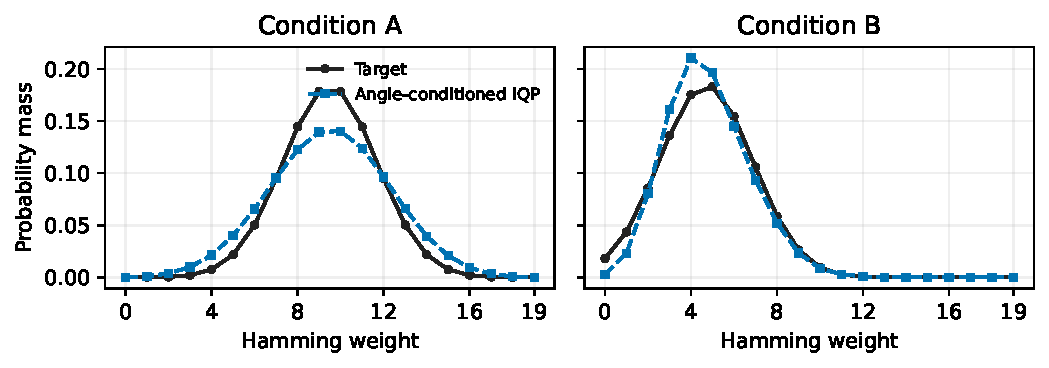
\includegraphics[width=0.88\textwidth]{../results/summary/weight_fit.pdf}
\caption{Legacy Gaussian motivation, regenerated from its archived ten-seed
study. One shared angle-conditioned checkpoint family changes its Hamming-
weight profile with the input; the no-condition output compromises. This is
not Ising evidence and does not override the failed novelty gate.}
\label{fig:legacy}
\end{figure}

Historical sparse-grid, condition-count, topology, ancilla, and negative
audits remain archived in the repository. A target-specific permutation twirl
can make Bitstring TVD equal profile TVD for a known distribution that is
uniform within Hamming shells, but it changes the output protocol and does not
show that the untwirled circuit learned the symmetry.  Those results are not
part of the present central evidence line and cannot rescue the blocked Ising
campaign.

\section{Reproducibility inventory}
\label{app:reproducibility}

The package provides the following independently inspectable layers:
\begin{enumerate}
\item a strict JSON manifest whose digest binds model, data, estimator,
training, statistical, and budget rules;
\item exact Ising coupling reconstruction, target enumeration, calibration,
and content-addressed target archives;
\item immutable gate records, reservations, result-bundle schemas, and
monotonic stage release;
\item deployment signatures, phase-feature maps, role-tagged datasets,
balanced training helpers, and exact-TV evaluation;
\item hierarchical bootstrap, benefit-retention, Oracle, interpolation, and
ancilla decision functions;
\item theorem-support, estimator-scaling, response-spectrum, campaign, and
manuscript audit tests; and
\item deterministic scripts for evidence figures, report tables, the main
manuscript, and this supplement.
\end{enumerate}

The central regeneration commands are:
\begin{verbatim}
uv sync --group dev
uv run pytest
uv run ruff check src scripts tests
uv run python scripts/prepare_ising_campaign.py --targets-only
uv run python scripts/run_ising_campaign.py --stage primary --dry-run
uv run python scripts/generate_quantum_draft_figures.py
uv run python scripts/run_estimator_scaling.py \
  --output /tmp/iqp-cond-estimator-scaling.json
uv run python scripts/audit_response_spectrum.py \
  --output /tmp/iqp-cond-response-spectrum.json  # blocked, exit 2
uv run python scripts/build_campaign_report.py
(cd paper && latexmk -pdf -interaction=nonstopmode \
  -halt-on-error main.tex)
\end{verbatim}
The target-only command rechecks existing exact archives and releases no gate.
The first theorem gate is already terminally failed.  Running either the full
preparation command or a downstream campaign CLI command returns a blocked
status before dataset generation, reservation, or trainer access.  The
repository does not contain or claim persistent Ising checkpoints.

\section{Adversarial review checklist}
\label{app:review}

Before any future external circulation, an independent quantum-information or
QML expert must review the proofs, closest-prior search, estimator scope, and
significance.  A new positive decision must not edit the existing failed gate;
it requires a new manifest version and evidence chain.  The following items
also remain mandatory:
\begin{itemize}
\item replace anonymous metadata and generic contribution/interest statements;
\item validate every DOI and arXiv version against the final bibliography;
\item rerun the complete suite and clean-environment regeneration;
\item inspect every rendered page for blanks, clipping, unresolved references,
and overfull boxes; and
\item archive independent review responses and allow major objections to
reopen the theorem, claims, experiments, or venue decision.
\end{itemize}
